\hypertarget{vec2d_8h}{
\section{vec2d.h File Reference}
\label{vec2d_8h}\index{vec2d.h@{vec2d.h}}
}
Define 2-d vectors and associated operations.  


{\tt \#include $<$cmath$>$}\par
{\tt \#include $<$blitz/tinyvec.h$>$}\par
{\tt \#include $<$blitz/tinyvec-et.h$>$}\par


Include dependency graph for vec2d.h:\nopagebreak
\begin{figure}[H]
\begin{center}
\leavevmode
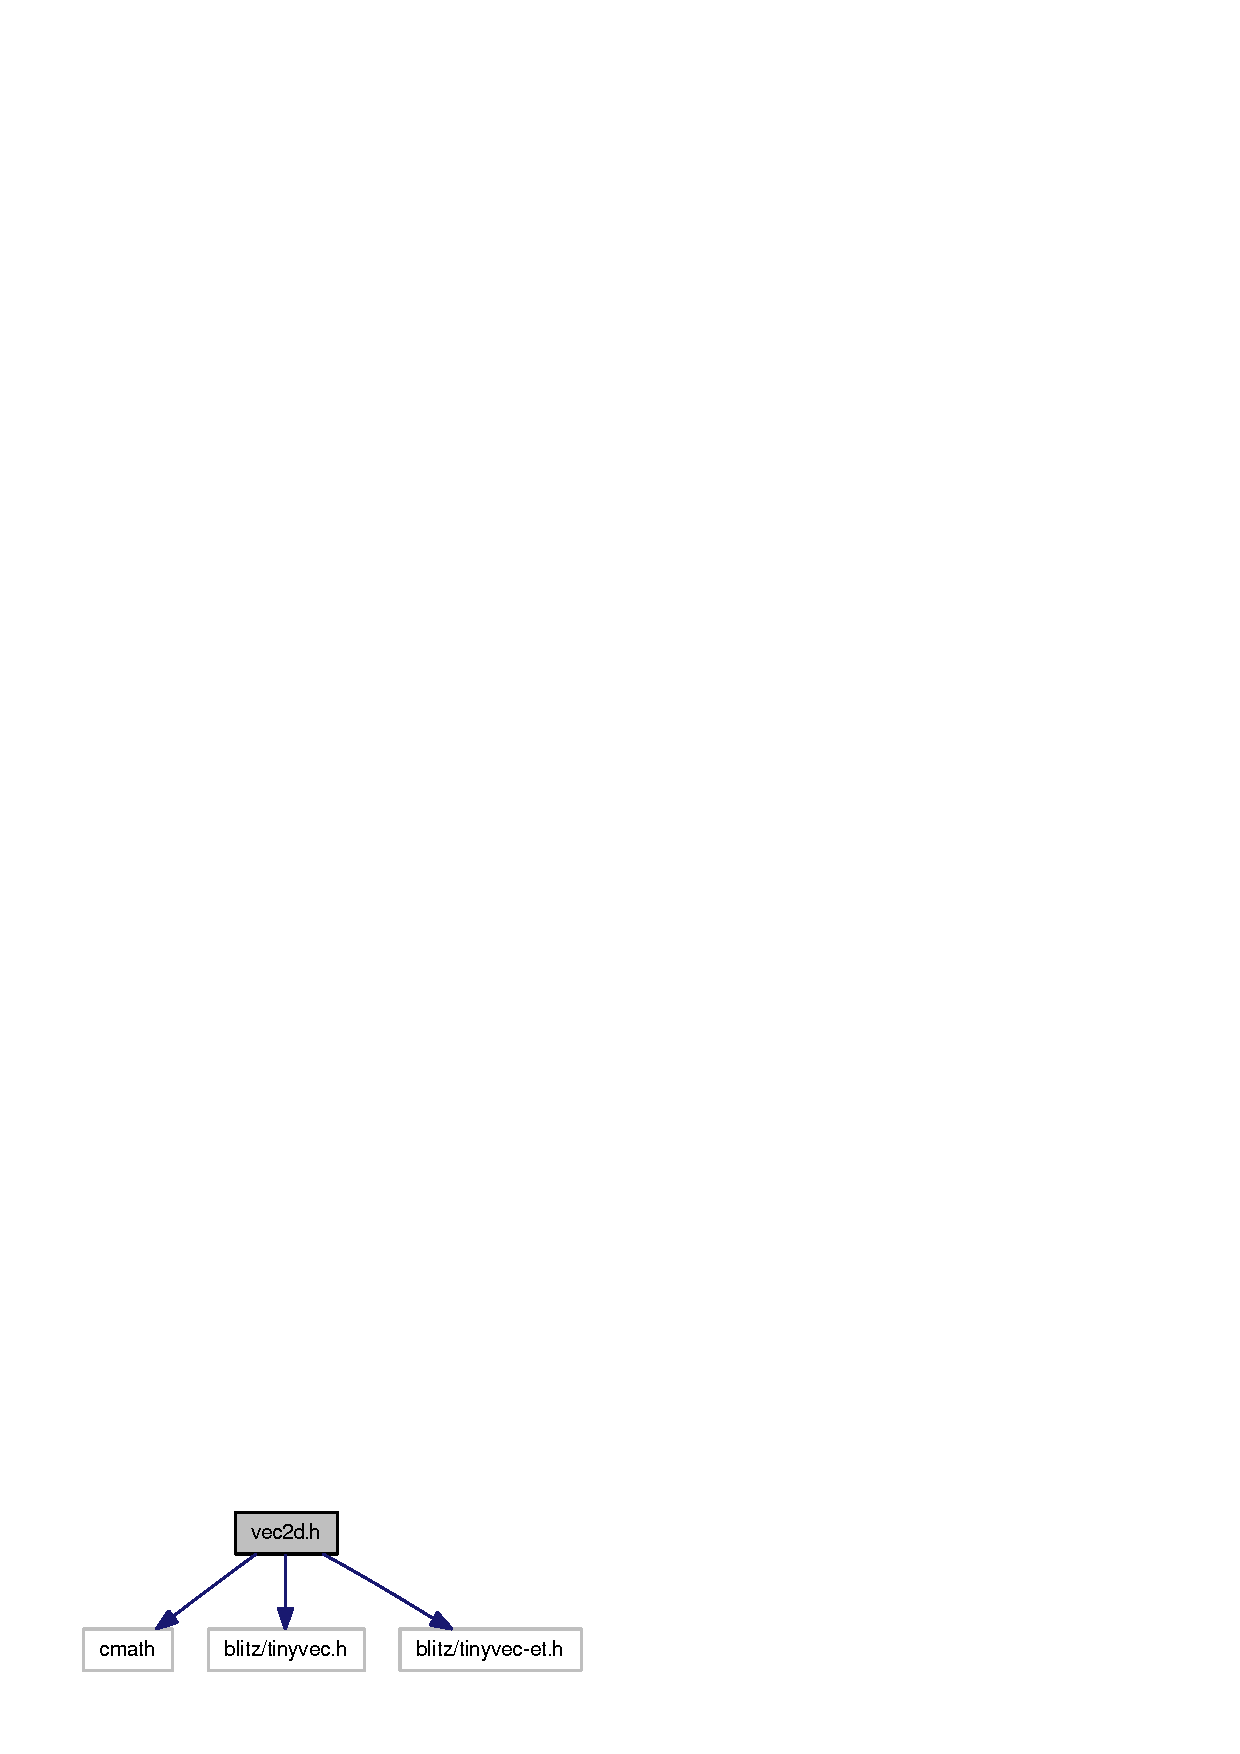
\includegraphics[width=141pt]{vec2d_8h__incl}
\end{center}
\end{figure}


This graph shows which files directly or indirectly include this file:\nopagebreak
\begin{figure}[H]
\begin{center}
\leavevmode
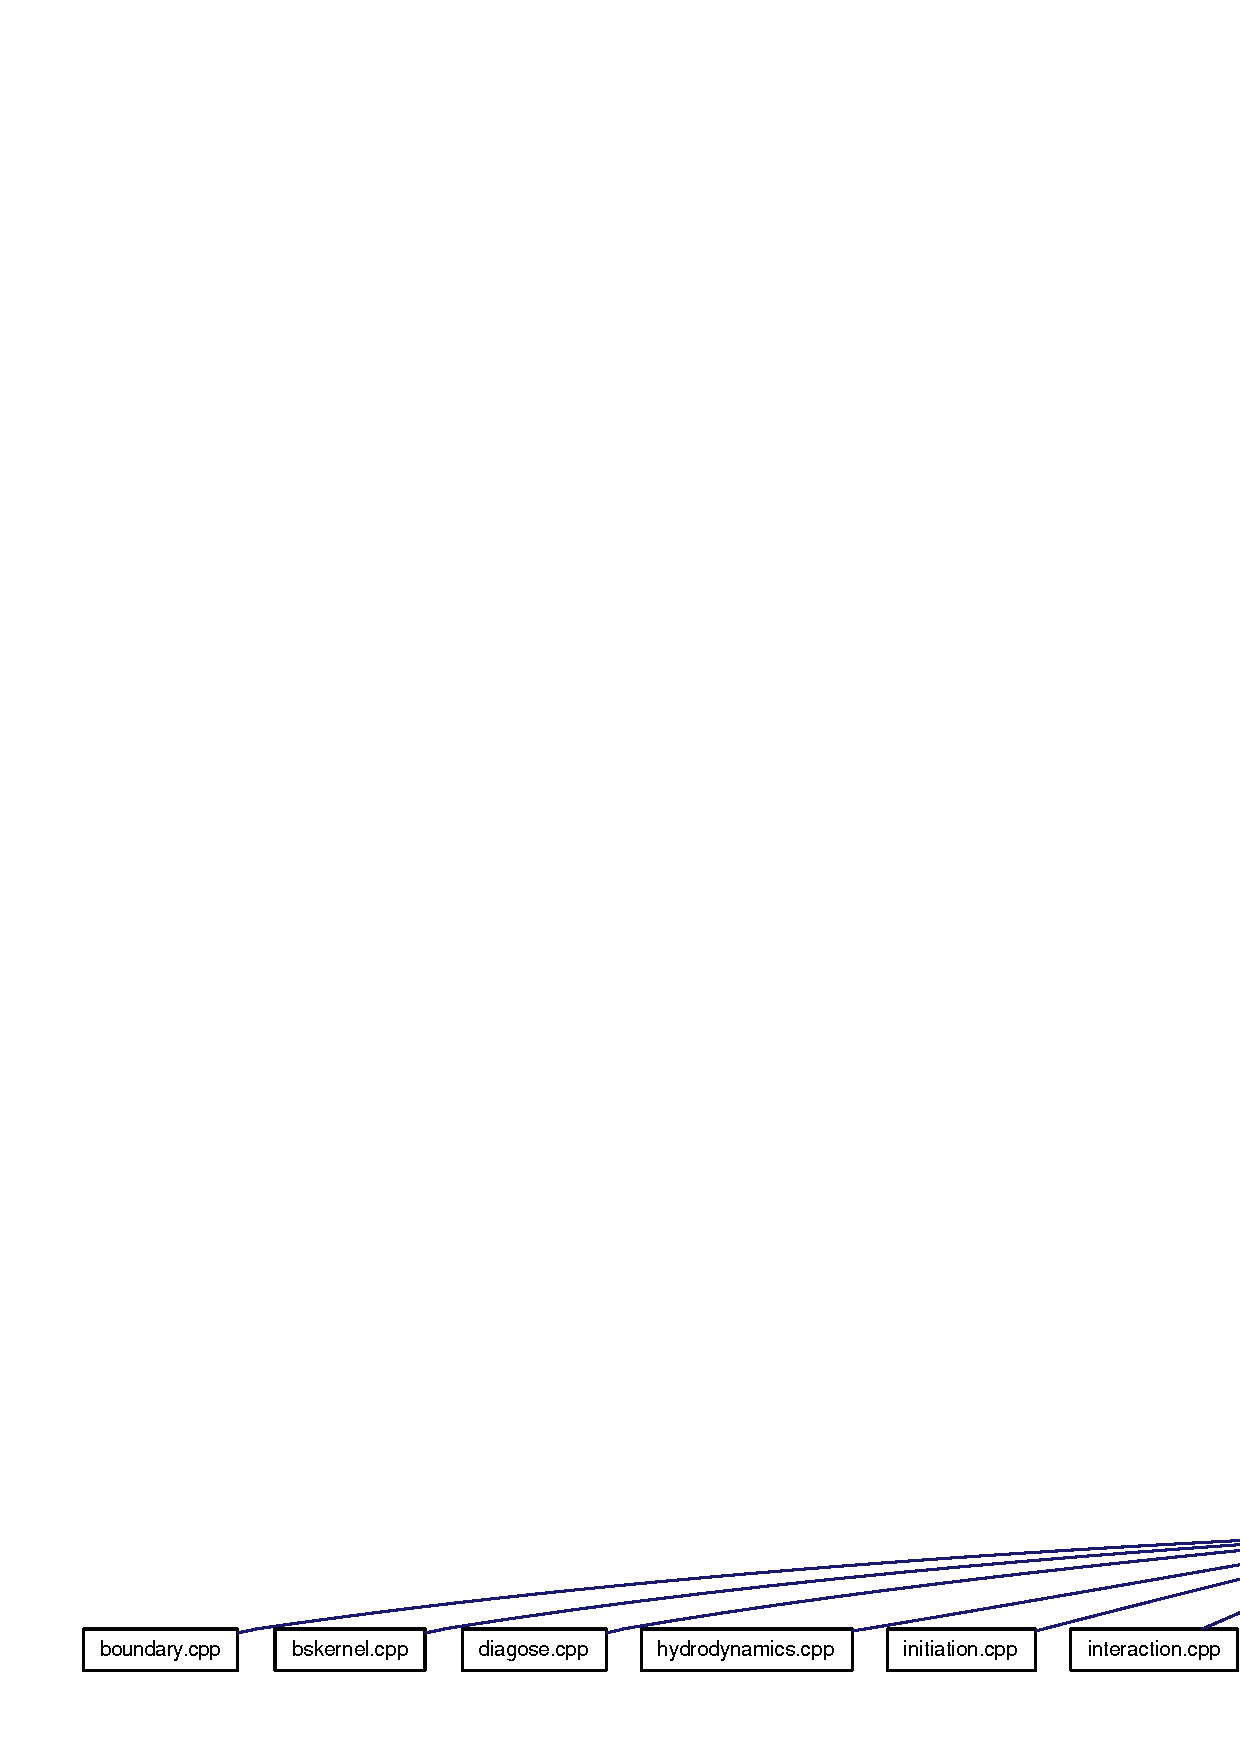
\includegraphics[width=420pt]{vec2d_8h__dep__incl}
\end{center}
\end{figure}
\subsection*{Typedefs}
\begin{CompactItemize}
\item 
\hypertarget{vec2d_8h_268cbe88997e7b383a3f73ea7b5822aa}{
typedef TinyVector$<$ double, 2 $>$ \textbf{Vec2d}}
\label{vec2d_8h_268cbe88997e7b383a3f73ea7b5822aa}

\end{CompactItemize}
\subsection*{Functions}
\begin{CompactItemize}
\item 
\hypertarget{vec2d_8h_d4fd110790320d1dd8d63411159b4d9c}{
double \hyperlink{vec2d_8h_d4fd110790320d1dd8d63411159b4d9c}{v\_\-abs} (const Vec2d \&v)}
\label{vec2d_8h_d4fd110790320d1dd8d63411159b4d9c}

\begin{CompactList}\small\item\em Return the absolute value of the vector (the length). \item\end{CompactList}\item 
\hypertarget{vec2d_8h_ce785ede99492e5a2e149d4a9a6521af}{
double \hyperlink{vec2d_8h_ce785ede99492e5a2e149d4a9a6521af}{v\_\-sq} (const Vec2d \&v)}
\label{vec2d_8h_ce785ede99492e5a2e149d4a9a6521af}

\begin{CompactList}\small\item\em Return the square sum of the vector values. \item\end{CompactList}\item 
\hypertarget{vec2d_8h_59971685b370dc9fe915f7d3ae23bf3b}{
double \hyperlink{vec2d_8h_59971685b370dc9fe915f7d3ae23bf3b}{v\_\-sqdiff} (const Vec2d \&v)}
\label{vec2d_8h_59971685b370dc9fe915f7d3ae23bf3b}

\begin{CompactList}\small\item\em Return the square difference of the vector values. \item\end{CompactList}\item 
double \hyperlink{vec2d_8h_977aa48c7b1ffeff460162482c21e2c4}{v\_\-distance} (const Vec2d \&va, const Vec2d \&vb)
\begin{CompactList}\small\item\em Return the distance of two points given as vectors. \item\end{CompactList}\item 
\hypertarget{vec2d_8h_5b8cbe588276a9c63c1fdc5322ec877e}{
void \hyperlink{vec2d_8h_5b8cbe588276a9c63c1fdc5322ec877e}{perodic\_\-position} (Vec2d \&va, const Vec2d \&vb, const Vec2d \&perodic)}
\label{vec2d_8h_5b8cbe588276a9c63c1fdc5322ec877e}

\begin{CompactList}\small\item\em Return the perodic position. \item\end{CompactList}\item 
\hypertarget{vec2d_8h_22f4e97ed7ca9e188dc4e074a1b2e5a7}{
double \textbf{sqr} (double x)}
\label{vec2d_8h_22f4e97ed7ca9e188dc4e074a1b2e5a7}

\end{CompactItemize}


\label{_details}
\hypertarget{_details}{}
\subsection{Detailed Description}
Define 2-d vectors and associated operations. 

\begin{Desc}
\item[Author:]Xiangyu Hu $<$\href{mailto:Xiangyu.Hu@aer.mw.tum.de}{\tt Xiangyu.Hu@aer.mw.tum.de}$>$ 

changes by: Martin Bernreuther $<$\href{mailto:Martin.Bernreuther@ipvs.uni-stuttgart.de}{\tt Martin.Bernreuther@ipvs.uni-stuttgart.de}$>$ 

changes by: Andreas Mattes \end{Desc}


\subsection{Function Documentation}
\hypertarget{vec2d_8h_977aa48c7b1ffeff460162482c21e2c4}{
\index{vec2d.h@{vec2d.h}!v\_\-distance@{v\_\-distance}}
\index{v\_\-distance@{v\_\-distance}!vec2d.h@{vec2d.h}}
\subsubsection[{v\_\-distance}]{\setlength{\rightskip}{0pt plus 5cm}double v\_\-distance (const Vec2d \& {\em va}, \/  const Vec2d \& {\em vb})\hspace{0.3cm}{\tt  \mbox{[}inline\mbox{]}}}}
\label{vec2d_8h_977aa48c7b1ffeff460162482c21e2c4}


Return the distance of two points given as vectors. 



return v\_\-abs(va-vb); double dx=va\mbox{[}0\mbox{]}-vb\mbox{[}0\mbox{]}; double dy=va\mbox{[}1\mbox{]}-vb\mbox{[}1\mbox{]}; 

Here is the caller graph for this function:\nopagebreak
\begin{figure}[H]
\begin{center}
\leavevmode
\includegraphics[width=408pt]{vec2d_8h_977aa48c7b1ffeff460162482c21e2c4_icgraph}
\end{center}
\end{figure}
